\section{Antecedentes Relevantes}

La automatización y el diseño generativo de circuitos analógicos mediante inteligencia artificial han cobrado especial relevancia en años recientes. Para situar el aporte de este trabajo, resulta indispensable analizar las metodologías propuestas en la literatura técnica reciente.

En primer lugar, \textbf{AnalogCoder} \cite{analogcoder} introdujo la propuesta de diseñar circuitos tratándolos como código ejecutable; en lugar de pedirle al modelo de lenguaje que describa un circuito en lenguaje natural, se le instruye para que escriba un script en Python capaz de generarlo. Al convertir el diseño en un programa ejecutable se reduce significativamente la ambigüedad de la síntesis y el netlist resultante puede simularse de inmediato. El sistema funciona sin necesidad de reentrenar el modelo base y comprueba recursivamente cada propuesta con una secuencia de verificaciones por simulación SPICE, validando que el circuito simule sin nodos flotantes, que los puntos de operación en corriente continua sean correctos y que la respuesta dinámica o de frecuencia cumpla con las especificaciones. Cuando una verificación falla, la traza de error regresa al modelo para orientar el siguiente intento de corrección. No obstante, esta aproximación coordina todo el flujo con un solo agente y se limita a nivel de transistor sobre un proceso de fabricación específico.

Por su parte, \textbf{AnalogAgent} \cite{analogagent} reparte esta carga de trabajo mediante un esquema de colaboración multiagente. Su contribución central consiste en la gestión y destilación del conocimiento acumulado durante los fallos: cuando un intento de diseño resulta fallido, el sistema procesa el error para traducirlo en una regla heurística explícita que se incorpora a una memoria auto-evolutiva y se recupera en iteraciones futuras, reduciendo el número total de llamadas al modelo. Adicionalmente, el estudio documenta una limitación típica de los agentes monolíticos basados en modelos de lenguaje: a medida que el historial de chat crece con cada intento de corrección, el resumen de contexto tiende a diluir u omitir detalles e instrucciones técnicas críticas. Esta estrategia de acumular conocimiento para guiar los pasos subsiguientes influye directamente en la concepción del agente curador de este trabajo, aunque mantiene la limitación de operar a nivel de transistor.

Finalmente, \textbf{CircuitLM} \cite{circuitlm} comparte con este proyecto el nivel de abstracción a nivel de componentes y módulos comerciales a partir de especificaciones de lenguaje natural. Este sistema emplea una tubería multiagente dedicada a la identificación de componentes, la consulta de hojas de especificaciones y la estructuración del esquema. No obstante, se orienta a electrónica digital y embebida ---microcontroladores como Arduino o ESP32--- y difiere del presente trabajo en su método de validación: en lugar de integrar simulación SPICE en el lazo, verifica la topología con un motor determinista de reglas eléctricas y un modelo de lenguaje supervisor. Sus propios autores señalan la verificación con simulador en el lazo como una limitación pendiente, justamente la señal de realimentación que este proyecto incorpora.

\section{Ubicación de este Proyecto}

\begin{figure}[htbp]
    \centering
    \makebox[\textwidth][c]{%
        \hspace*{-1cm}% Compensación del margen izquierdo para simetría visual
        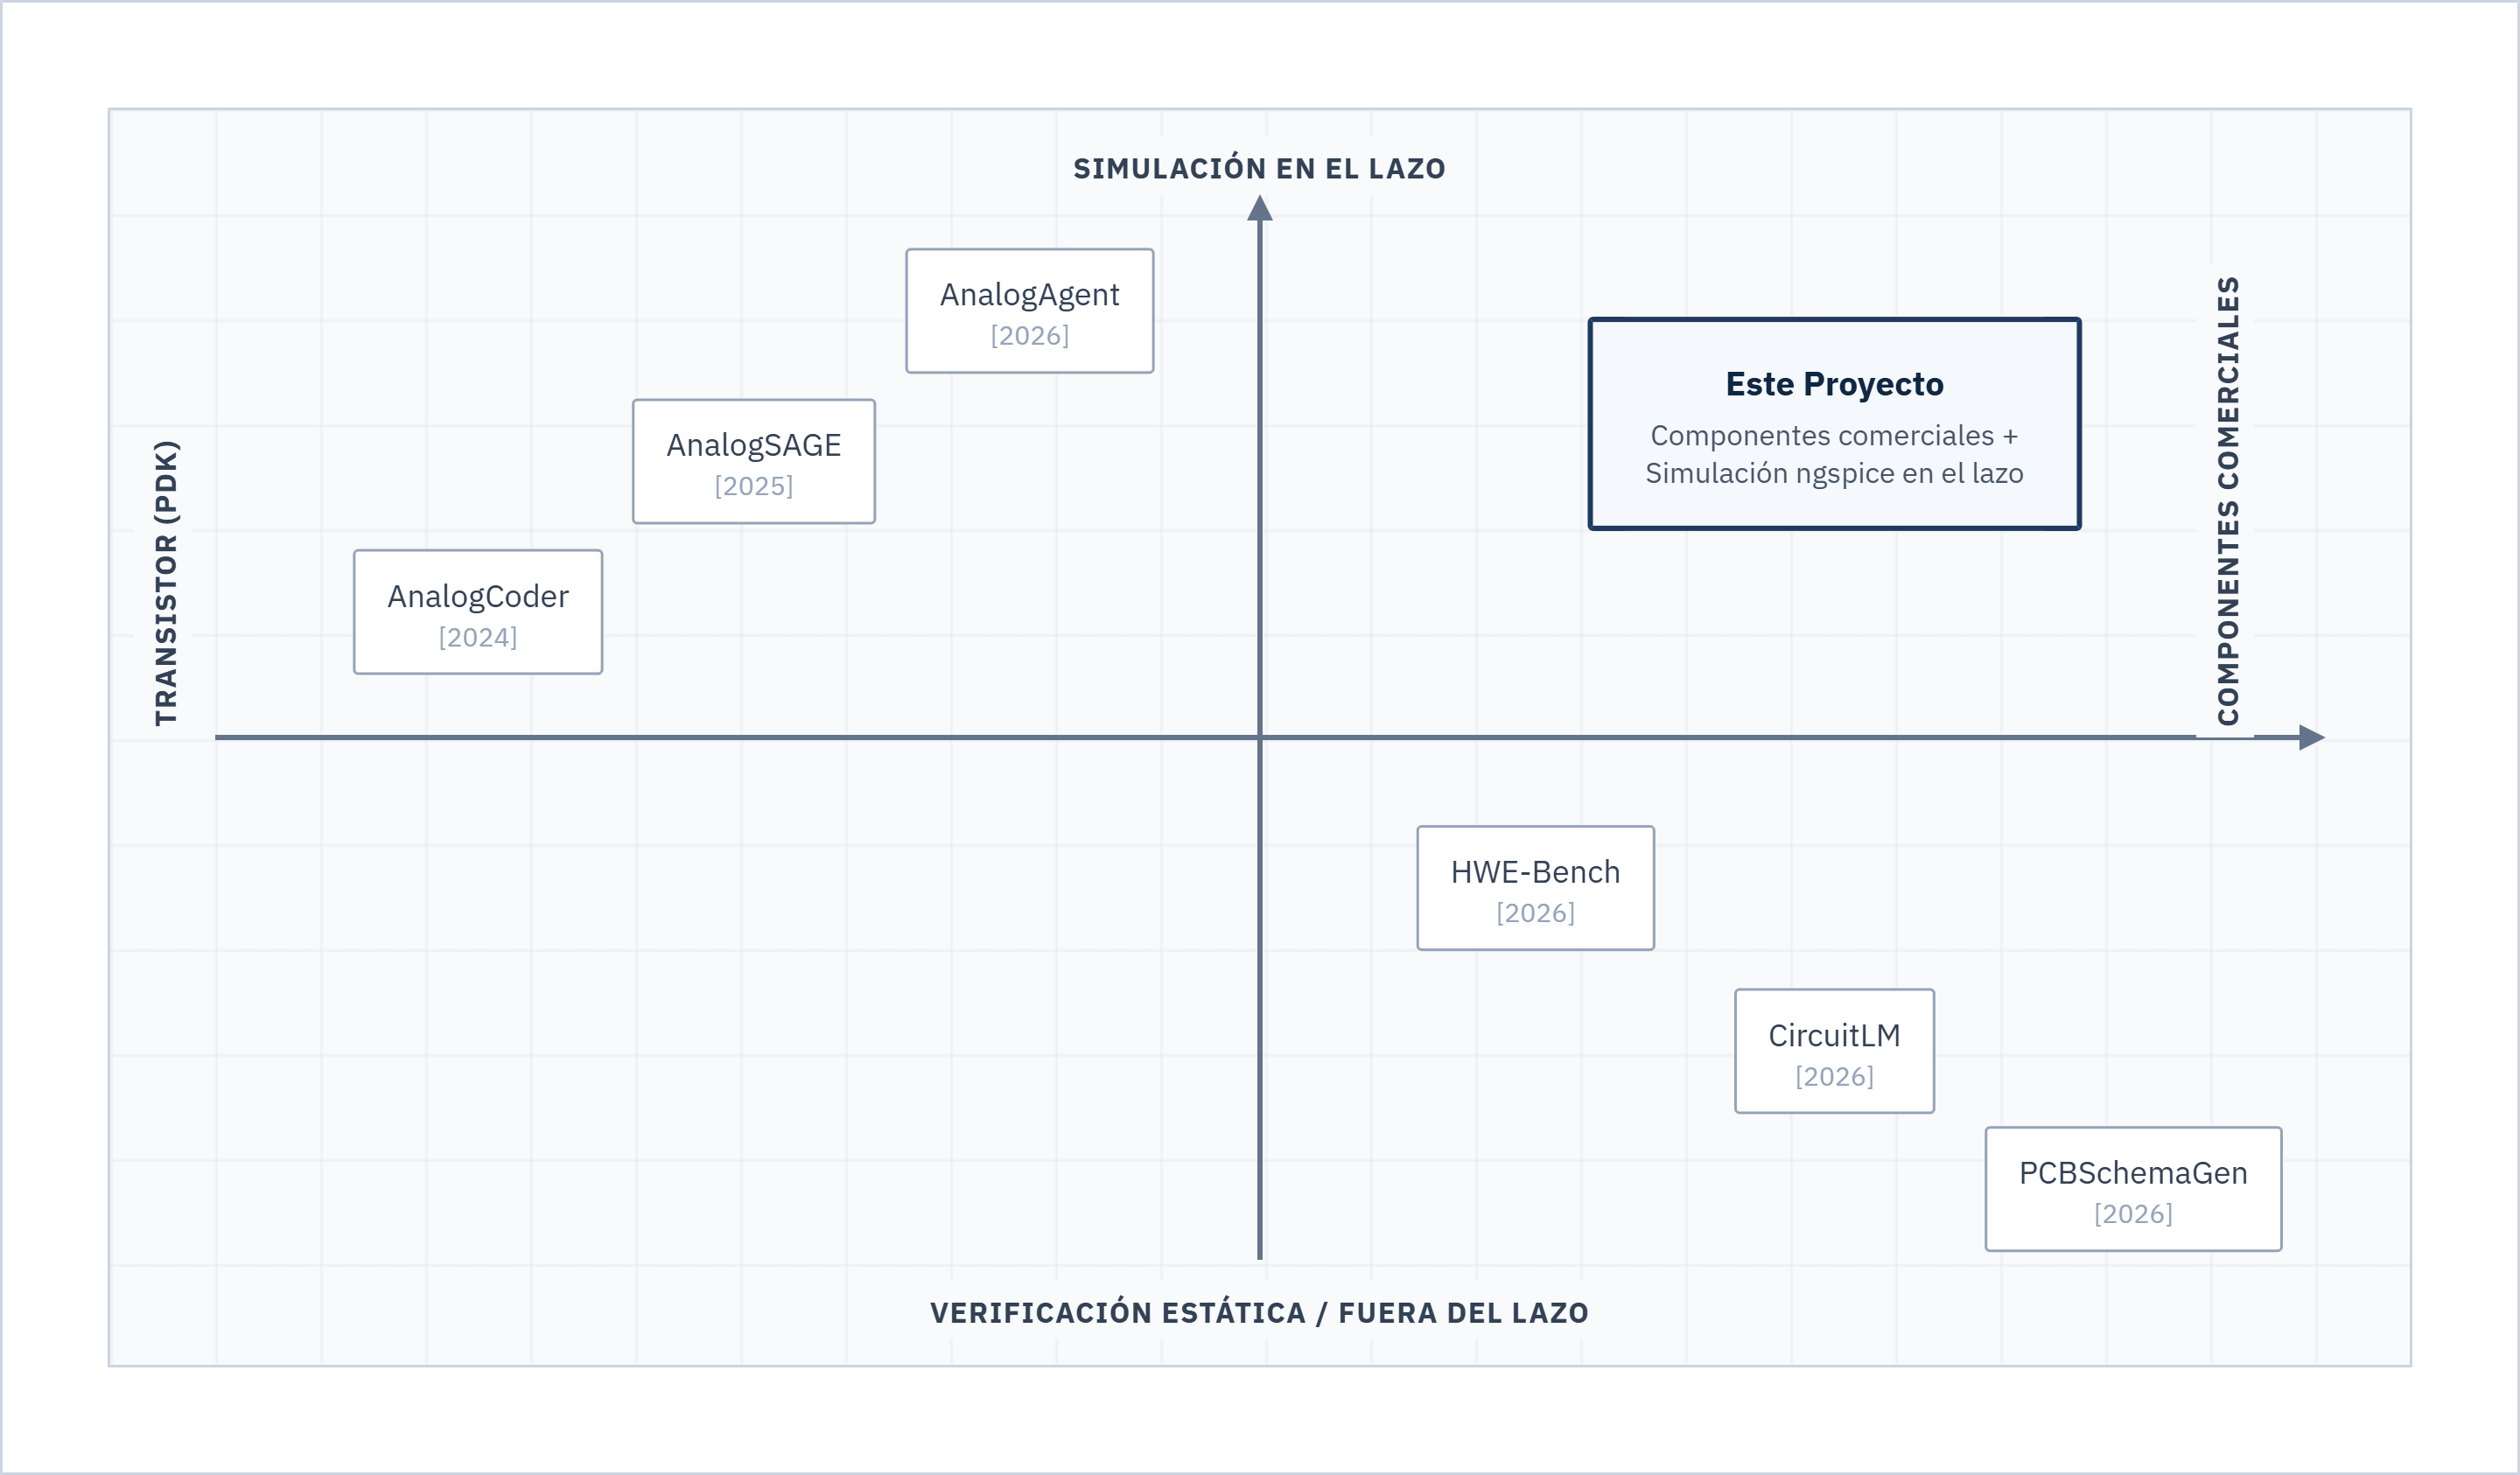
\includegraphics[width=1.2\textwidth, trim=0cm 0cm 0cm 0cm, clip]{../src/diagrams/edo_arte.png}%
    }
    \caption{Posición de los trabajos revisados según cuatro rasgos.}
    \label{fig:comparacion_estado_arte}
    \vspace{0.3cm}
\end{figure}

Junto a los desarrollos mencionados, otras propuestas complementan el panorama del área. \textbf{AnalogSAGE} \cite{analogsage} introduce memoria estratificada y mecanismos de autoevolución a la síntesis a nivel de transistor; \textbf{PCBSchemaGen} \cite{pcbschemagen} extiende la verificación estática de reglas al ámbito de tarjetas de circuito impreso reales; y \textbf{HWE-Bench} \cite{hwebench} provee un entorno de evaluación comparativa que mide el rendimiento de netlists generados contrastándolos con diseños de referencia de expertos a través de simulaciones SPICE. Adicionalmente, se registran contribuciones como \textbf{ADO-LLM} \cite{adollm} para la optimización bayesiana en el diseño físico y \textbf{SPICEPilot} \cite{spicepilot} para la generación asistida de scripts de control.

La Figura \ref{fig:comparacion_estado_arte} organiza los trabajos según los dos ejes que mejor los distinguen: el nivel de abstracción del diseño ---de transistor a componentes comerciales--- y la función de la simulación en el flujo ---de la verificación estática a la realimentación en el lazo---. El esquema de coordinación y el mecanismo de optimización paramétrica complementan el contraste y se desarrollan en el texto.

Al contrastar las soluciones se observa que ninguno de los antecedentes recopilados integra simultáneamente los cuatro rasgos propuestos en este ecosistema. Mientras que los sistemas orientados a transistores explotan la simulación en lazo cerrado y el ajuste paramétrico iterativo, no contemplan el uso de componentes comerciales. Por el contrario, los enfoques comerciales evitan la simulación dinámica en el lazo de optimización o la reducen a una métrica de prueba externa. Este proyecto une la retroalimentación física por simulación de los flujos a nivel de transistor con el diseño a nivel de placa mediante componentes comerciales, implementando una arquitectura multiagente coordinada por un curador entrenado por aprendizaje por refuerzo.


\begin{table}[h!]
\centering
\small
\label{tab:estado_del_arte}
\vspace{0.3cm}

\setlength{\aboverulesep}{0pt}
\setlength{\belowrulesep}{0pt}
\renewcommand{\arraystretch}{1.5}
\setlength{\extrarowheight}{5pt}
\arrayrulecolor{guinda}
\rowcolors{1}{white}{rowgray}

% Estructura rígida basada en tabularx con alineación vertical al centro
\begin{tabularx}{\textwidth}{
  >{\centering\arraybackslash}m{2.6cm} 
  >{\centering\arraybackslash}m{2.4cm} 
  >{\raggedright\arraybackslash}X 
  >{\centering\arraybackslash}m{1.5cm}
}
\toprule
\rowcolor{guinda}
\textcolor{white}{\textbf{Nombre del Paper}} & 
\textcolor{white}{\textbf{Origen}} & 
\textcolor{white}{\textbf{Descripción}} & 
\textcolor{white}{\textbf{Enlace}} \\ 
\midrule

AnalogCoder & 
\worldflag{HK} \worldflag{US} \newline \footnotesize HK / EE. UU. & 
Primer agente LLM sin entrenamiento para diseño de circuitos analógicos mediante generación de código Python y bibliotecas de subcircuitos. & 
\href{https://arxiv.org/abs/2405.14918}{\textbf{[Link]}} \\

AnalogAgent & 
\worldflag{SG} \newline \footnotesize Singapur & 
Arquitectura multi-agente con memoria auto-evolutiva que aprende de los fallos de simulación sin depender de bibliotecas externas. & 
\href{https://arxiv.org/abs/2603.23910}{\textbf{[Link]}} \\ 

CircuitLM & 
\worldflag{BD} \newline \footnotesize Bangladesh & 
Tubería multiagente que genera esquemas a nivel de placa con componentes comerciales, orientada a electrónica digital y embebida; valida con un motor de reglas eléctricas (ERC) y un modelo supervisor, sin simulación en el lazo. & 
\href{https://arxiv.org/abs/2601.04505}{\textbf{[Link]}} \\

\bottomrule
\end{tabularx}
\caption{Resumen - Estado del Arte}
\end{table}